\documentclass{beamer}
\mode<presentation>
{
	\usetheme{CambridgeUS}
	\usecolortheme{rose} %seagull
	\usefonttheme[onlylarge]{structuresmallcapsserif}
	%\setbeamercovered{transparent}	
}

\usepackage[utf8]{inputenc}
\usepackage{graphicx}
\usepackage[export]{adjustbox}
\usepackage{subfig}
\usepackage{amsmath}
\usepackage[spanish]{babel}


\AtBeginSection[]{
	\begin{frame}
		\vfill
		\centering
		\begin{beamercolorbox}[sep=8pt,center,shadow=true,rounded=true]{title}
			\usebeamerfont{title}\insertsectionhead\par%
		\end{beamercolorbox}
		\vfill
	\end{frame}
}


\title[Rigidez y Visualización]{Rigidez de ovaloides y visualización computacional}
\author{Eva María González García}
\date{18 de diciembre de 2018}
\institute[UGR]{Universidad de Granada}

\begin{document}
	
	
	\begin{frame}
		\maketitle
	\end{frame}
	
	\begin{frame}
		\frametitle{Índice}
		\tableofcontents
	\end{frame}
	
	
	\section{Rigidez de ovaloides}
	
	\subsection{Isometrías y rigidez}
	
	\begin{frame}
		\frametitle{¿Qué es una isometría?}
		\begin{block}{Definición}
			Dadas dos superficies S y $S'$ y dada una aplicación $f : S \longrightarrow S'$, diremos que $f$ es una \textbf{isometría} (local) si:
			\begin{itemize}
				\item es un difeomorfismo (difeomorfismo local)
				\item conserva la primera forma fundamental, esto es: $\;\;\;\;\;\;\;\;\;\;\;\;\;\;\;\;\;\;\;\;\;$ $\forall p \in S$, $\forall u,v \in T_p S$. $\langle df_p(u), df_p(v)\rangle = \langle u, v\rangle$
			\end{itemize}
		\end{block}
		${ }$\\
		\begin{block}{Proposición}
			$f : S \to S'$ es una isometría local si y sólo si conserva la longitud de las curvas.
		\end{block}
	\end{frame}
		
	\begin{frame}
		\frametitle{¿Qué es una superficie rígida?}
		\begin{block}{Definición}
			Diremos que $S \subset \mathbb{R}^3$ es una \textbf{superficie rígida} cuando toda isometría $f : S \to S'$ es la restricción de un movimiento rígido, es decir, existe un movimiento rígido $F : \mathbb{R}^3 \to \mathbb{R}^3$ tal que $f = F_{|S}$.
		\end{block}
		${ }$\\
		\begin{figure}[h]
			\begin{center}
				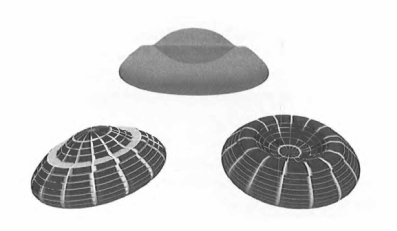
\includegraphics[width=0.55\textwidth]{imagenes/no_rigid}
			\end{center}
		\end{figure}
	\end{frame}
	
	
	\subsection{Rigidez de la esfera}
	
	\begin{frame}
		\frametitle{La esfera es rígida}
		\begin{figure}[h]
			\begin{center}
				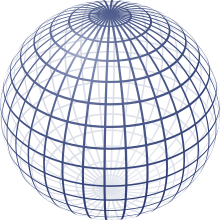
\includegraphics[width=0.2\textwidth]{imagenes/sphere.png}
			\end{center}
		\end{figure}
		${ }$\\
		\begin{block}{Teorema de rigidez de la esfera}
			Consideremos una esfera de radio $r>0$, $\mathbb{S}^2(r)$, y $S$ una superficie conexa cualquiera. En esta situación toda isometría $f : \mathbb{S}^2(r) \to S$ es la restricción de un movimiento rígido de $\mathbb{R}^3$. En particular, $S$ es una esfera de igual radio que la de partida.
		\end{block}
	\end{frame}
	
	\begin{frame}
		\frametitle{Resultados para la rigidez}
		Los siguientes resultados se usan para demostrar la rigidez de la esfera.
		\begin{block}{Teorema Egregium de Gauss}
			Sean $f : S \to S'$ una isometría local entre dos superficies y $K$ y $K'$ sus respectivas curvaturas de Gauss. Entonces, $K = K'\circ f$.
		\end{block}
		Los siguientes resultados son también utilizados para demostrar la rigidez de los ovaloides.
		\begin{block}{Teorema de Hilbert-Liebmann}
			La única superficie conexa y compacta con curvatura de Gauss constante es la esfera.
		\end{block}
	\end{frame}
	
	\begin{frame}
		\frametitle{Isometrías y movimientos rígidos}
		
		\begin{itemize}
			\item Demostramos una versión simplificada del Teorema fundamental de la teoría local de superficies.
			\item Esta simplificación es suficiente para la demostración de la rigidez de los ovaloides.
		\end{itemize}
		
		
		
		
		\begin{block}{Teorema fundamental para superficies compactas}
			Dadas dos superficies $S$ y $S'$ orientables y compactas.
			Si $f : S \to S'$ es una isometría que conserva la segunda forma fundamental, entonces existe un movimiento rígido $\Phi : \mathbb{R}^3 \to \mathbb{R}^3$ tal que $\Phi_{\mid S} = f$.
		\end{block}
	\end{frame}
	
	
	\subsection{Rigidez de ovaloides}
	
	\begin{frame}
		\frametitle{Ovaloides}
		\begin{itemize}
			\item Motivación: generalizar la rigidez de la esfera.
		\end{itemize}
		${ }$\\
		\begin{block}{Definición}
			Llamaremos \textbf{ovaloide} a una superficie $S \subset \mathbb{R}^3$ compacta y conexa cuya curvatura de Gauss sea siempre positiva.
		\end{block}
	\end{frame}
	
	\begin{frame}
		\frametitle{Ejemplos de ovaloides}
		\begin{figure}[h]
			\subfloat[$\frac{x^2}{a^2}+\frac{y^2}{b^2}+\frac{z^2}{c^2}=1$]{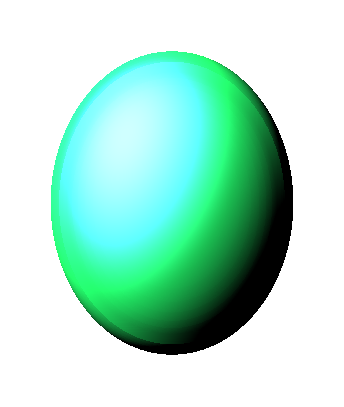
\includegraphics[width=0.3\linewidth]{imagenes/Prueba2t.png}}
			\subfloat[$x^4+y^4+z^4=1$]{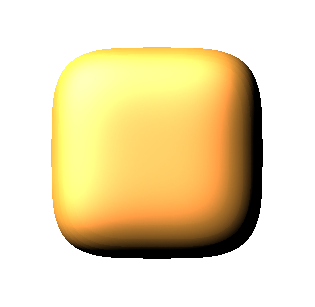
\includegraphics[width=0.3\linewidth]{imagenes/Ovaloidt.png}}
			\subfloat[$12x^2 + 12z^2 + 22y^2 + 8xy^2=1$ ]{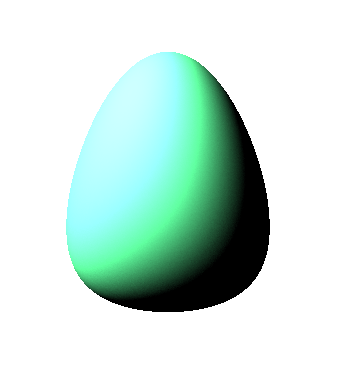
\includegraphics[width=0.3\linewidth]{imagenes/granvilleegg.png}}
		\end{figure}
%		Imagen de ovaloides teselados.
	\end{frame}
	
	\begin{frame}
		\frametitle{Propiedades de los Ovaloides}
		\begin{itemize}
			\item Convexos.
			\begin{block}{Teorema de Hadamard-Stoker}
				Sea un ovaloide $S \subset \mathbb{R}^3$ y $\Omega$ su dominio interior. Entonces:
				
				\begin{enumerate}
					\item Para todo $x, y \in \overline{\Omega}$. Entonces, $]x, y[ \subset \Omega$. En particular, $\Omega$ es convexo.
					\item Para cada $p \in S$, $\Pi_p \cap S = \{p\}$, donde $\Pi_p$ es el plano tangente afín a $S$ en p. Además, $\overline{\Omega} \subset \bigcap_{p \in S} \; \Pi^{+}_{p}$.
				\end{enumerate}
			\end{block}
		\end{itemize}
		

		${ }$\\
	\end{frame}
	
	\begin{frame}
		\frametitle{Teorema de Cohn-Vossen}
		\framesubtitle{Los ovaloides son rígidos}
		\begin{block}{Teorema de rigidez de Cohn-Vossen}
			Sean $S$ y $S'$ ovaloides. Entonces, cualquier isometría $f : S \to S'$ es restricción de un movimiento rígido de $\mathbb{R}^3$.
		\end{block}
		${ }$\\
		Demostración:
		\begin{itemize}
			\item $A(f)_p = -(df)^{-1}_{p} \circ (dN')_{f(p)} \circ (df)_p$
			\item Teorema Egregium de Gauss.
			\item Fórmula de Minkowski.
			\item Integral de Herglotz.
			\item Probar que $(dN')_{f(p)} \circ (df)_p = (df)_p \circ (dN)_p$.
			\begin{itemize}
				\item $A(f)_p = -(dN)_p$
			\end{itemize}
			\item Teorema fundamental de la teoría local de superficies.
		\end{itemize}
	\end{frame}
	
	\begin{frame}
		\frametitle{Demostración parte 1}
		
		
		La fórmula de Minkowski nos dice que:
		\begin{itemize}
			\item $\int_S H = - \int_S \langle p, N(p) \rangle K(p) dp$
		\end{itemize}
		
		Sea el endomorfismo $A(f)_p = -(df)^{-1}_{p} \circ (dN')_{f(p)} \circ (df)_p$, se tiene que:
		\begin{itemize}
			\item $tr \; A(f)_p$ = $2(H' \circ f)$ y $det \; A(f)_p$ = $K' \circ f$.
		\end{itemize}
		
		Por el teorema Egregium de Gauss, $det \; A(f)_p = K' \circ f = K$:
		
		\begin{itemize}
			\item $2 \int_S H = - \int_S \langle p, N(p) \rangle det(dN)_p dp - \int_S \langle p, N(p) \rangle det A(f)_p dp$
		\end{itemize}
		
		La fórmula de Herglotz nos dice que:
		\begin{itemize}
			\item $2 \int_S H' \circ f = \int_S \langle p, N(p) \rangle [tr(dN)_p trA(f)_p - tr(dN)_p A(f)_p] dp$
		\end{itemize}
		Restando las dos igualdades:
		\begin{itemize}
			\item $2 \int_S (H' \circ f - H)(p) dp = $
			
			$\int_S \langle p, N(p) \rangle [tr(dN)_p trA(f)_p - tr(dN)_p A(f)_p + det(dN)_p + det A(f)_p] dp$
		\end{itemize}
	\end{frame}
	
	\begin{frame}
		\frametitle{Demostración parte 2}
		
		Para dos endormorfismos autoadjuntos $\Phi$ y $\Psi$ se cumple:
		\begin{itemize}
			\item $tr \; \Phi \; tr \; \Psi - tr \; (\Phi \circ \Psi) + det \; \Phi + det \; \Psi = det \; (\Phi + \Psi)$
		\end{itemize}
		
		Sustituyendo en la ecuación anterior:
		\begin{itemize}
			\item $2 \int_S (H' \circ f - H)(p) dp = \int_S \langle p, N(p) \rangle det[A(f)_p + (dN)_p] dp$
		\end{itemize}
		
		Por el teorema de Hadamard-Stoker, para $N$ normal interior:
		\begin{itemize}
			\item $\forall q \in \Omega. \; h_p (q) = \langle p - q, N(p)\rangle < 0$
		\end{itemize}
		Para $\Phi$ definido positivo y $\Psi$ definido negativo con $det \; \Phi = det \; \Psi$:
		\begin{itemize}
			\item $det \; (\Phi + \Psi) \leq 0$ y $det \; (\Phi + \Psi) = 0 \iff \Phi = - \Psi$
		\end{itemize}
		Por tanto:
		$\int_S (H' \circ f - H)(p) \; dp = \int_S \langle p, N(p) \rangle det[A(f)_p + (dN)_p] \; dp \geq 0$
		
	\end{frame}
	
	\begin{frame}
		\frametitle{Demostración parte 3}
		
		Aplicamos lo obtenido a $f^{-1}$:
		\begin{itemize}
			\item $\int_{S'} (H \circ f^{-1} - H')(p) \; dp \geq 0$
		\end{itemize}
		Por la fórmula del cambio de variable ($\int_{S_2} \Phi = \int_{S_1} (\Phi \circ F)|Jac \Phi|$):
		\begin{itemize}
			\item $\int_S (H - H' \circ f) (p) \; dp \geq 0$
		\end{itemize}
		
		Por tanto:
		$\int_S (H' \circ f - H)(p) \; dp = \int_S \langle p, N(p) \rangle det[A(f)_p + (dN)_p] \; dp \leq 0$
		
		${ }$\\
		
		Por la igualdad, $det[A(f)_p + (dN)_p]=0$ y por el lema:
		\begin{itemize}
			\item $A(f)_p = -(dN)_p = -(df)^{-1}_{p} \circ (dN')_{f(p)} \circ (df)_p$
		\end{itemize}
		
		
		${ }$\\
		
		Por tanto, $(dN')_{f(p)} \circ (df)_p = (df)_p \circ (dN)_p$ $\forall p \in S$
		
		\begin{block}{Lema}
			Sea $S$ y $S'$ dos superficies, $f: S \to S'$ una isometría, si $f$ cumple $(dN')_{f(p)} \circ (df)_p = (df)_p \circ (dN)_p$ $\forall p \in S$. Entonces, $f$ conserva la segunda forma fundamental.
		\end{block}

		
	\end{frame}


	

	
	
	\section{Visualización computacional}
	\subsection{Visualización por computador}
	
	\begin{frame}
		\frametitle{Aplicaciones de la visualización computacional}
		\begin{itemize}
			\item Videojuegos
			\item Cine
			\item Visualización científica y técnica
			\item Diseño 3D
			\item Simulación
		\end{itemize}
	\end{frame}
	
	\begin{frame}
		\frametitle{Dos métodos de síntesis de imágenes}
		\begin{itemize}
			\item Ray-tracing
				\begin{itemize}
					\item Lanzado de rayos y cálculo de intersecciones
					\item Resultados más realistas
					\item Más lento, aplicación: Cine, diseño 3D, efectos especiales...
				\end{itemize}
				${ }$\\
			\item Rasterización
				\begin{itemize}
					\item Mallas de triángulos y proyección 2D
					\item Más rápido, aplicación: Videojuegos, realidad virtual...
				\end{itemize}
		\end{itemize}
	\end{frame}
	
	\subsection{Ray-Tracing}
	
	\begin{frame}
		\frametitle{Rayos, cámara e imagen}
		\begin{figure}[h]
			\begin{center}
				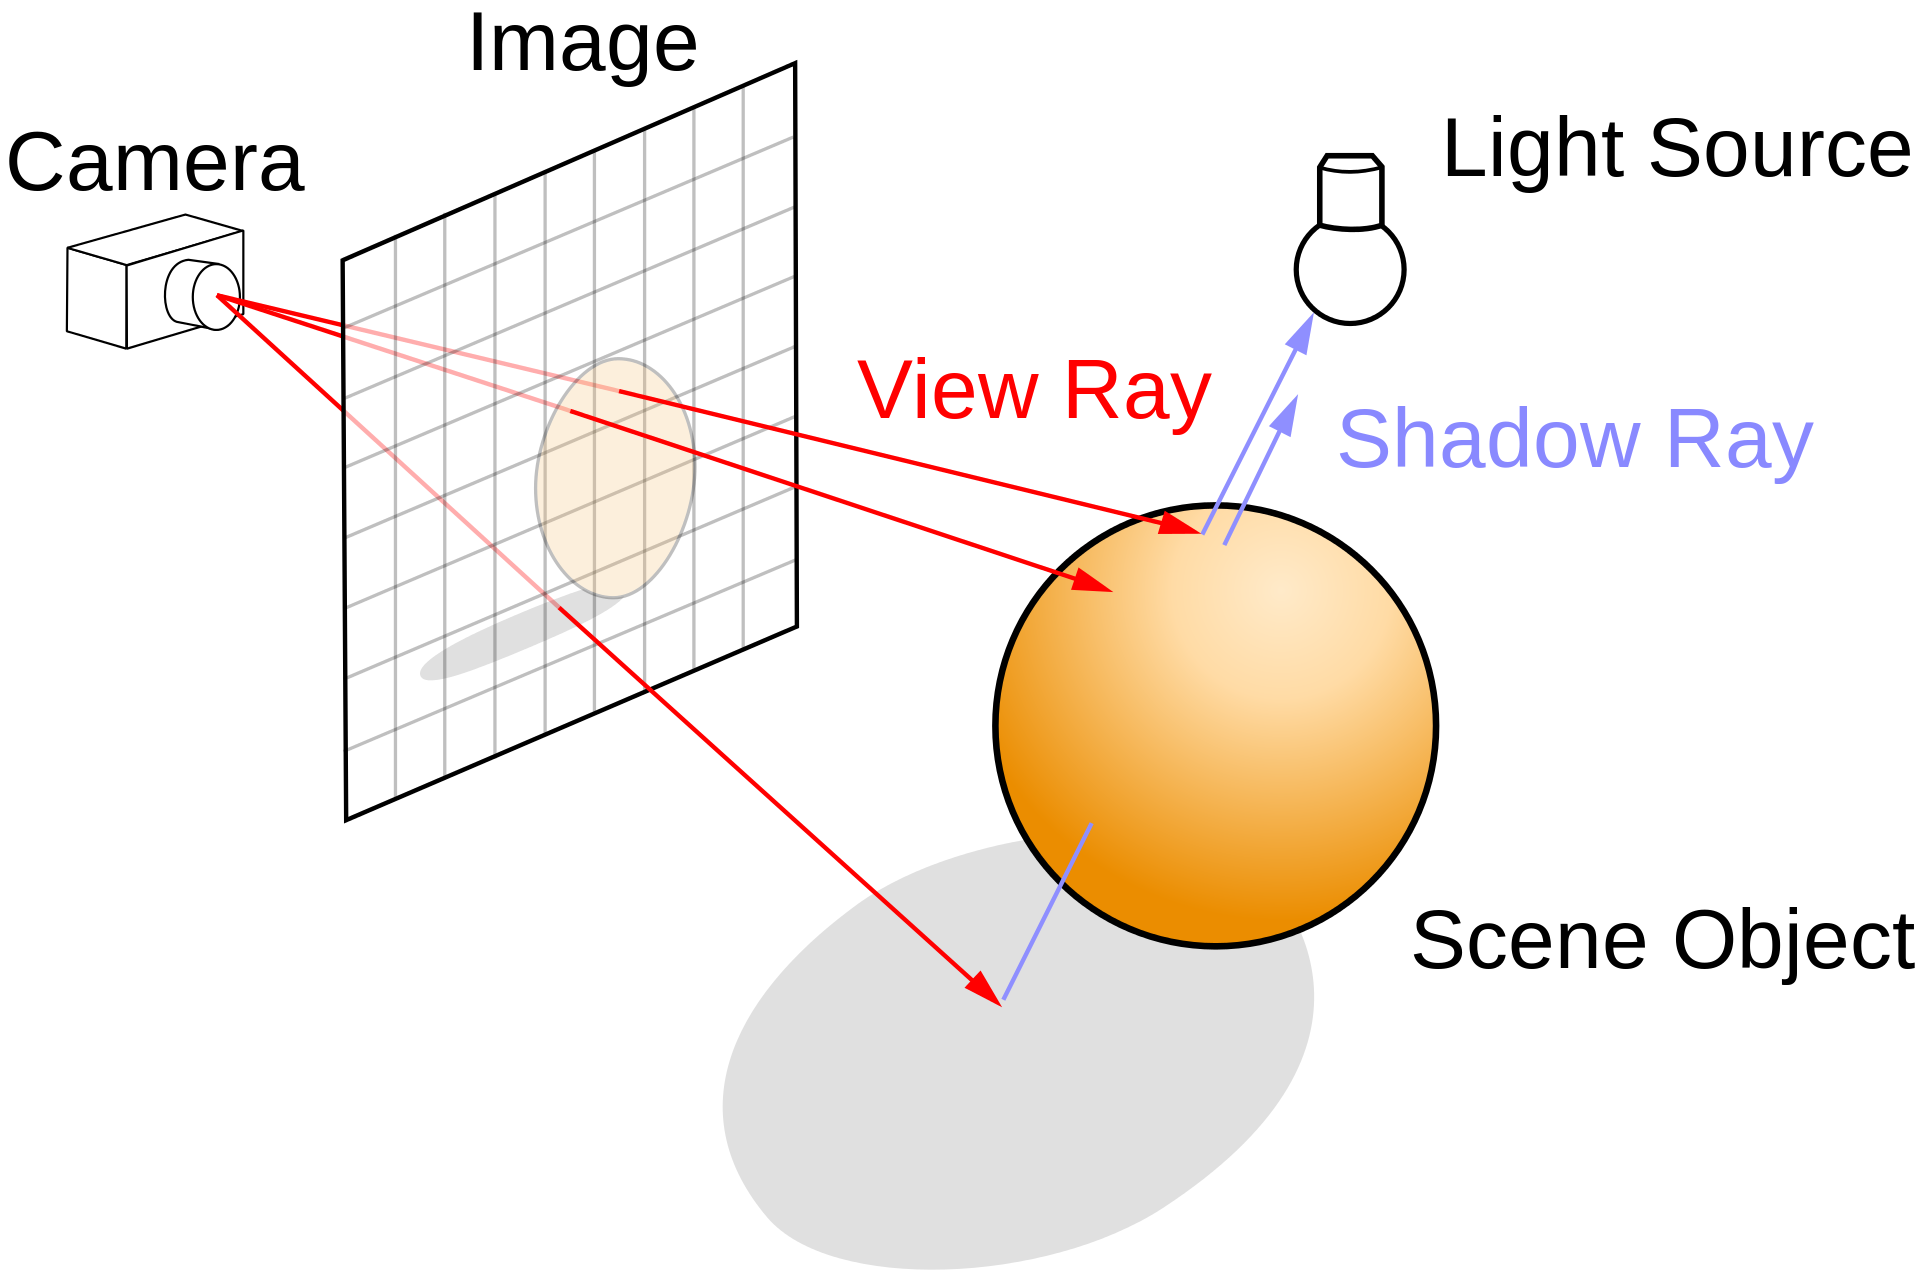
\includegraphics[width=0.55\textwidth]{imagenes/tracing}
			\end{center}
		\end{figure}
		${ }$\\
		Expresión:
		\begin{itemize}
			\item Rayos: $r(t)=o+dt$
			\item Superficies: $F(x,y,z)=0$
		\end{itemize}
	\end{frame}
	
	\begin{frame}
		\frametitle{Intersección de rayos con objetos}
		\framesubtitle{Intersección Rayo-Esfera}
		
		Ecuación de la esfera:
		${ }$\\
		\begin{itemize}
			\item $(p-c)\cdot(p-c) - R^2 = 0$
		\end{itemize}
		${ }$\\
		
		\begin{figure}[h]
				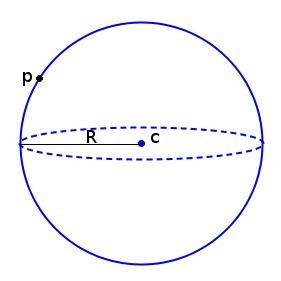
\includegraphics[width=0.35\textwidth]{imagenes/esfera}
		\end{figure}
		
	\end{frame}
	
	\begin{frame}
		\frametitle{Intersección de rayos con objetos}
		\framesubtitle{Intersección Rayo-Esfera}
		
		
		Intersección con rayos:
		${ }$\\
		
		\begin{itemize}
			\item Componiendo: $(o+td-c)\cdot(o+td-c) - R^2 = 0$
			
			${ }$\\
			
			\item Agrupando: $(d\cdot d)t^2 + 2d\cdot (o-c)t + (o-c)\cdot(o-c) - R^2 = 0$
			\begin{itemize}
				\item Es de la forma $At^2+Bt+C=0$
			\end{itemize}
			${ }$\\
			\item Resolviendo: $t = \frac{-B\pm \sqrt{B^2-4CA}}{2A}$
		\end{itemize}
	\end{frame}
	
	\begin{frame}
		\frametitle{Intersección de rayos con objetos}
		\framesubtitle{Intersección Rayo-Cubo}
		
		\begin{figure}[h]
			
\includegraphics[width=0.8\textwidth]{imagenes/Imagen2}
		\end{figure}
	\end{frame}
	
	\begin{frame}
		\frametitle{Iluminación}
		\framesubtitle{Ley de Lambert}
		
		\begin{itemize}
			\item $L = ER(\textbf{n}\cdot \textbf{l})$
			\item Color resultante del pixel = L + Sumando especular
		\end{itemize}
		
		${ }$\\
		
		\begin{figure}[h]
			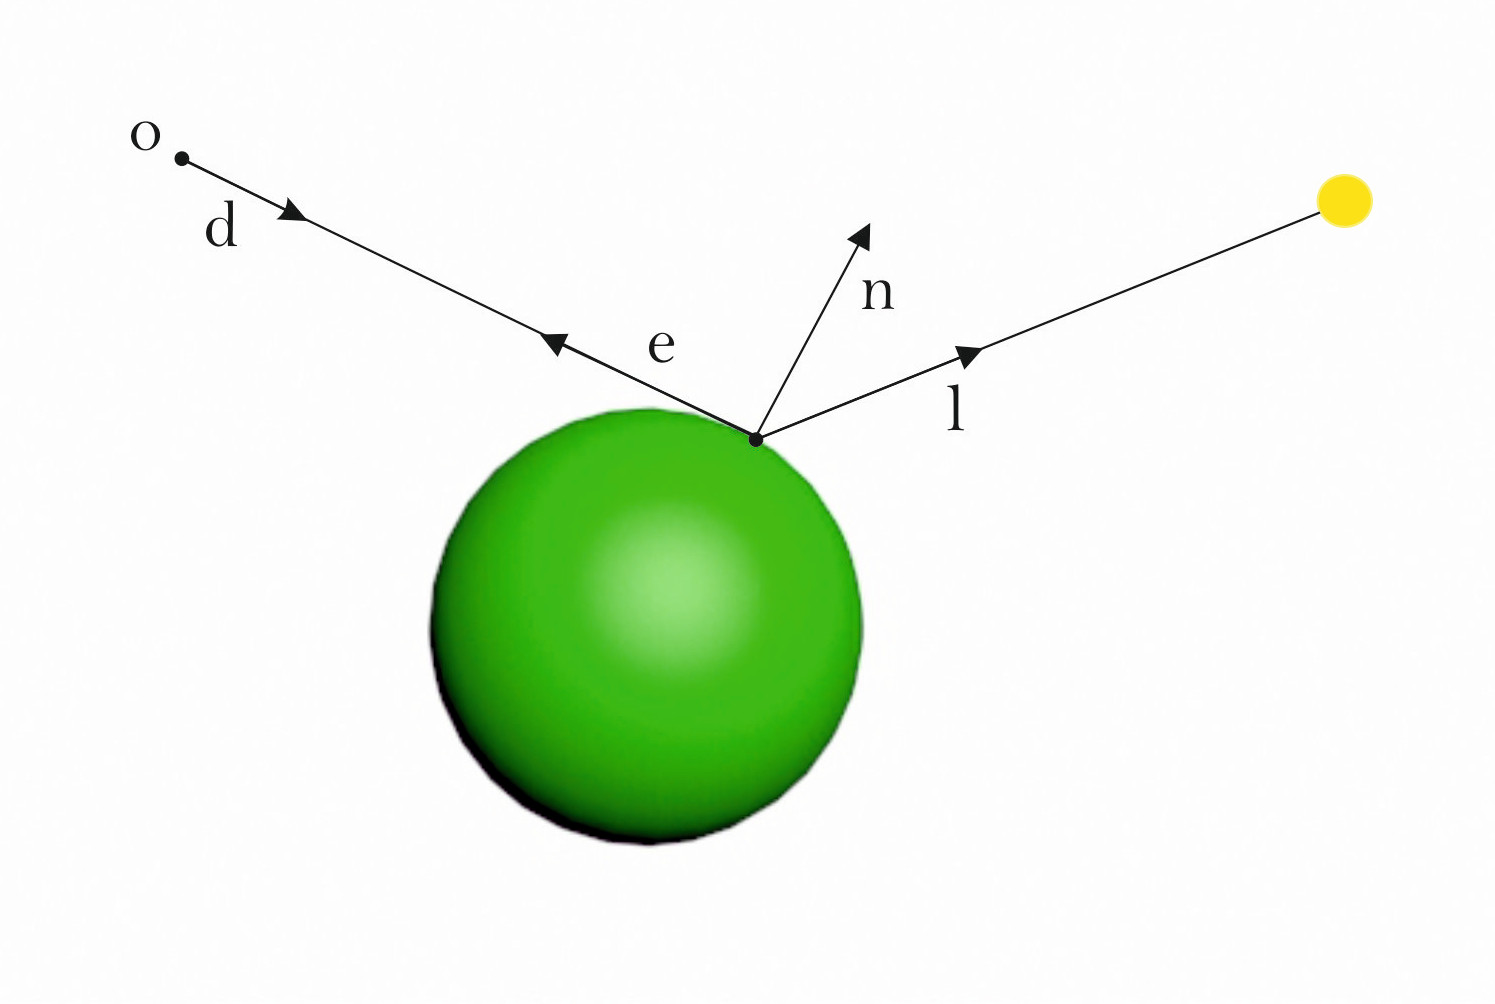
\includegraphics[width=0.6\textwidth]{imagenes/Imagen3t}
		\end{figure}
		
	\end{frame}
	
	\begin{frame}
		\frametitle{Iluminación}
		\framesubtitle{Componente especular del modelo de Phong}
		
		Sumando especular = CompEspecular * d *  $[max(0, Reflejado \cdot e)]^{expBrillo}$
		
		Donde, d = 0 si $n \cdot l$ es negativo, 1 en otro caso.
		
		${ }$\\
		
		\begin{figure}[h]
			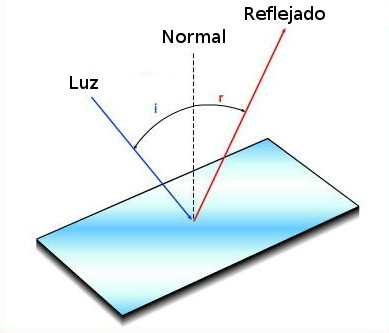
\includegraphics[width=0.5\textwidth]{imagenes/reflexion_luz}
		\end{figure}
		
	\end{frame}
	
	\begin{frame}
		\frametitle{Iluminación}
		\framesubtitle{Más de un objeto}
		
		\begin{figure}[h]
			
\includegraphics[width=0.8\textwidth]{imagenes/Imagen4}
		\end{figure}
		
	\end{frame}
	
	\subsection{Ray-Marchig}
	
	\begin{frame}
		\frametitle{Métodos iterativos de aproximación de soluciones}
		
		\begin{itemize}
			\item Imposibilidad de encontrar las soluciones de una ecuación de forma directa
			
			${ }$\\
			
			\item Necesidad de métodos iterativos que se aproximen a la solución
			\begin{itemize}
				\item Newton-Raphson
				\item Regula-Falsi
			\end{itemize}
			
			${ }$\\
			
			\item Combinación de métodos
		\end{itemize}
	\end{frame}
	
	\begin{frame}
		\frametitle{Newton-Raphson}
		
		\begin{itemize}
			\item Convergencia rápida
			\item No está asegurada la convergencia
		\end{itemize}
		
		\begin{figure}[h]
			\begin{center}
				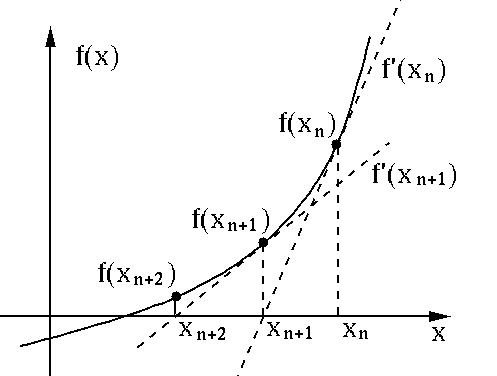
\includegraphics[width=0.9\textwidth]{imagenes/newton.png}
			\end{center}
		\end{figure}
	\end{frame}
	
	\begin{frame}
		\frametitle{Regula-Falsi}
		
		\begin{itemize}
			\item Converge más lentamente
			\item La convergencia está asegurada
			\begin{itemize}
				\item Teorema de los ceros de Bolzano
			\end{itemize}
		\end{itemize}
		
		\begin{figure}[h]
			\begin{center}
				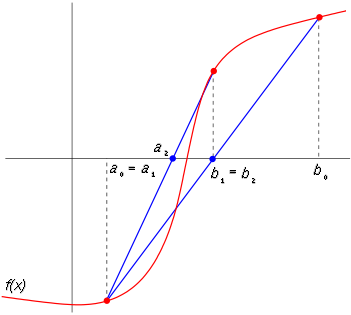
\includegraphics[width=0.45\textwidth]{imagenes/regulaF.png}
			\end{center}
		\end{figure}
		
	\end{frame}

	
	\begin{frame}
		\frametitle{Combinación de métodos}
		
		\begin{itemize}
			\item \textbf{Paso 0:} Tomar un intervalo inicial $[a_0, b_0]$ y una aproximación inicial $x_0$.
			
			${ }$\\
			\item \textbf{Paso 1:} Calcular el siguiente elemento de la sucesión mediante $x_{n+1} = x_n - \frac{f(x_n)}{f'(x_n)}$.
			${ }$\\
			\begin{itemize}
				\item Si $f(x_{n+1}) = 0$, hemos terminado.
				\item Si $x_{n+1}$ esta dentro del intervalo $[a_n, b_n]$:
				${ }$\\
				\begin{itemize}
					\item Si $f(a_n) \cdot f(x_{n+1}) < 0$, $b_n = x_{n+1}$.
					\item Si $f(b_n) \cdot f(x_{n+1}) < 0$, $a_n = x_{n+1}$.
				\end{itemize}
				${ }$\\
				\item Si $x_{n+1}$ está fuera del intervalo $[a_n, b_n]$ desestimamos $x_{n+1}$ y lo volvemos a calcular mediante $x_{n+1} = \frac{a_n f(b_n) - b_n f(a_n)}{f(b_n) - f(a_n)}$. De nuevo:
				${ }$\\
				\begin{itemize}
					\item Si $f(a_n) \cdot f(x_{n+1}) < 0$, $b_n = x_{n+1}$.
					\item Si $f(b_n) \cdot f(x_{n+1}) < 0$, $a_n = x_{n+1}$.
				\end{itemize}
			\end{itemize}
		\end{itemize}
	\end{frame}
	
	
	\begin{frame}
		\frametitle{Imágenes de prueba}
		
		\begin{figure}[h]
			\subfloat[Hiperboloide de una sola hoja]{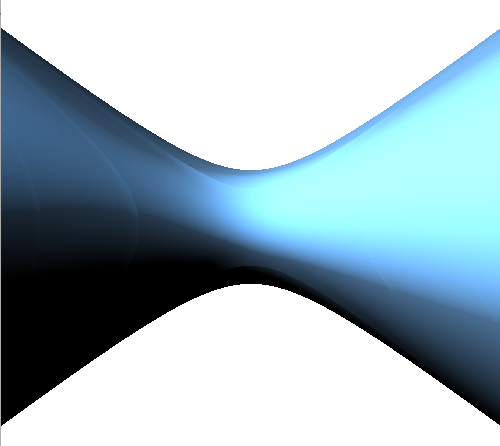
\includegraphics[width=0.5\linewidth]{imagenes/cuadricat.png}}
			\subfloat[Toro]{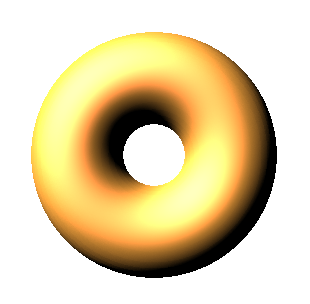
\includegraphics[width=0.5\linewidth]{imagenes/Torot.png}}
		\end{figure}
	\end{frame}
\end{document}